\section{Webservices}
\label{sec:Webservices}
Ein Webservice ist eine Technologie um Daten über standardisierte Internet-Protokolle zu übertragen.
Das Interface ermöglicht es dem Client (dem Anwender) mit dem Server über sog. \acs{HTTP}- oder auch \acs{HTTPS}-Requests zu kommunizieren.
Jeder Webservice hat eine spezifische Aufgabe, die auch als Funktion bezeichnet wird, die von einem oder mehreren Usern benutzt werden kann.
Um einen Webservice aufzurufen, muss dieser zunächst auf einem Webserver wie z.B. einem Tomcat-Server platziert werden.
Ein weiterer Vorteil eines Webservices ist, dass er eine plattformunabhängige Kommunikation ermöglicht.
D.h., dass er sowohl unter Linux als auch unter Windows verwendet werden kann.
Typische Einsatzgebiete eines Webservices sind z.B. der Austausch von Informationen über die Auslastung einer Reise, einer Liste von Bestellungen etc. (siehe Abbildung \vref{fig:webservice}).

\begin{figure}[h]
	\centering 
	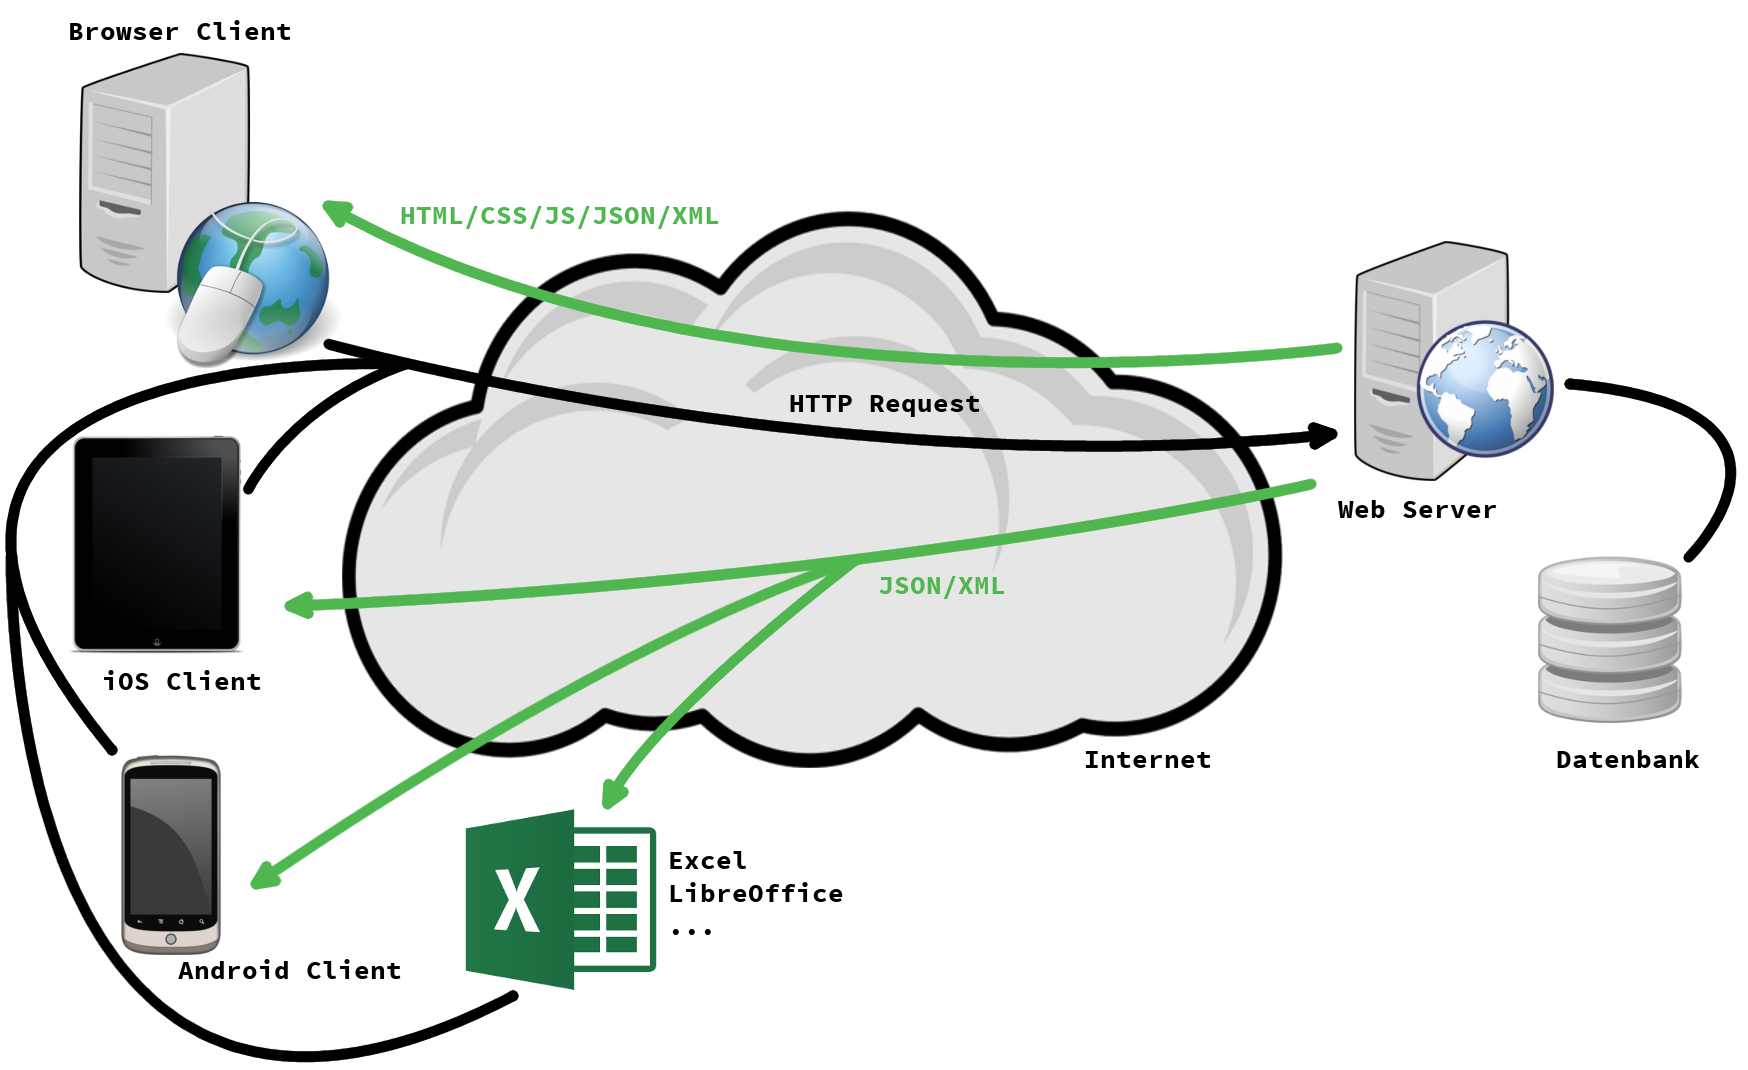
\includegraphics[width=0.6\textwidth]{img/webservice.png}
	\captionsetup{format=hang}
	\caption[Prinzip eines Webservice]{\label{fig:webservice}Prinzip eines Webservice \\Quelle: https://www.ransoft.at/images/others/webservice.png}
\end{figure}